\documentclass[12pt,a4paper]{article}
\usepackage[T2A]{fontenc}
\usepackage[utf8]{inputenc}
\usepackage[russian]{babel}
\usepackage{amsmath, amssymb}
\usepackage{graphicx}
\usepackage{hyperref}
\usepackage{listings}
\usepackage{xcolor}
\usepackage{geometry}
\usepackage{float}
\usepackage{caption}
\usepackage{enumitem}
\usepackage{titlesec}
\usepackage{fancyhdr}
\usepackage{array}
\usepackage{booktabs}

\geometry{a4paper, left=2.5cm, right=1.5cm, top=2cm, bottom=2cm}

\titleformat{\section}{\Large\bfseries}{\thesection}{1em}{}
\titleformat{\subsection}{\large\bfseries}{\thesubsection}{1em}{}

\lstset{
    language=Python,
    basicstyle=\ttfamily\small,
    keywordstyle=\color{blue},
    commentstyle=\color{green!40!black},
    stringstyle=\color{red},
    breaklines=true,
    frame=single,
    captionpos=b,
    showstringspaces=false,
    tabsize=4
}

\pagestyle{fancy}
\fancyhf{}
\fancyhead[L]{Лабораторная работа №1: Проектирование AI-сервиса на FastAPI}
\fancyhead[R]{\thepage}

\hypersetup{colorlinks=true, linkcolor=black, urlcolor=blue}

\begin{document}

\begin{titlepage}
    \begin{center}
        \textbf{МИНИСТЕРСТВО НАУКИ И ВЫСШЕГО ОБРАЗОВАНИЯ РОССИЙСКОЙ ФЕДЕРАЦИИ}
        \vspace{0.5cm}

        \textbf{Федеральное государственное автономное образовательное учреждение \\ высшего образования}
        \vspace{0.3cm}

        \textbf{«НАЦИОНАЛЬНЫЙ ИССЛЕДОВАТЕЛЬСКИЙ ТЕХНОЛОГИЧЕСКИЙ УНИВЕРСИТЕТ МИСИС»}
        \vspace{2cm}

        \textbf{Институт компьютерных наук}
        \vspace{0.3cm}

        \textbf{Кафедра Инженерной кибернетики}
        \vspace{1cm}

        \textbf{ОТЧЁТ}\\
        \textbf{по лабораторной работе №1}
        \vspace{0.3cm}

        \textbf{по дисциплине «Современные интеллектуальные сетевые сервисы»}
        \vspace{1.5cm}

        \huge{\textbf{Проектирование AI-сервиса \\ на FastAPI}}
        \vspace{2cm}
    \end{center}

    \begin{flushright}
        \textbf{Выполнил:} \\
        Студент группы \underline{МПИ-25-1-2} \\
        Мефедов А.М. \\
        \vspace{0.5cm}
        \textbf{Проверил:} \\
        Преподаватель \\
        Корнет М.Е. \\
        \vspace{2cm}
        \textbf{Оценка:} \hrulefill
    \end{flushright}

    \begin{center}
        \vfill
        Москва, 2026
    \end{center}
\end{titlepage}

\tableofcontents
\newpage

% ============================================================
\section{Цель работы}

Научиться проектировать программную архитектуру AI-сервиса, использующего модель машинного обучения, определить место API в общей ИИ-системе и реализовать REST API на FastAPI, изучив основные принципы программного взаимодействия между AI-моделью и внешними информационными системами.

В качестве предметной области рассматривается сервис \textbf{агроскоринга} банка: по сведениям о сельскохозяйственном предприятии (регион, площадь посевов, культура, погодные показатели, история платежей, задолженность) сервис рассчитывает числовую оценку риска, категорию риска и рекомендацию оператору банка.

% ============================================================
\section{Архитектура API}

\subsection{Потребители сервиса}

API проектируется как единая точка входа для нескольких потребителей: CRM банка, веб-портала, мобильного приложения, внутренних банковских сервисов и BI-системы. Все они взаимодействуют с сервисом по протоколу HTTP, формат обмена данными --- JSON. Потребителям достаточно знать контракт API (OpenAPI-спецификацию); детали реализации модели от них скрыты.

\subsection{Порядок обработки запроса на прогноз}

Обработка запроса \texttt{POST /predict} проходит следующие этапы:

\begin{enumerate}
    \item \textbf{Структурная валидация} (Pydantic, схема \texttt{FarmRequest}) --- проверка типов, обязательности полей и диапазонов значений. При ошибке --- HTTP 422, расчёт риска не выполняется.
    \item \textbf{Проверка готовности модели} --- если модель недоступна, возвращается HTTP 503.
    \item \textbf{Бизнес-валидация} --- регион должен входить в справочник \{Krasnodar, Rostov, Stavropol\}. При ошибке --- HTTP 400.
    \item \textbf{Расчёт риска} --- модель (\texttt{RiskModel.predict()}) возвращает \texttt{risk\_score} $\in [0; 1]$.
    \item \textbf{Постпроцессинг} --- преобразование score в категорию (\texttt{low} $< 0.3 \le$ \texttt{medium} $< 0.7 \le$ \texttt{high}) и формирование рекомендации.
    \item \textbf{Сохранение} результата в хранилище под уникальным \texttt{request\_id} (UUID4).
    \item \textbf{Логирование} запроса и результата (\texttt{farm\_id}, \texttt{request\_id}, score, уровень риска).
    \item \textbf{Формирование ответа} по схеме \texttt{PredictionResponse}.
\end{enumerate}

\subsection{Синхронные и асинхронные операции}

Расчёт прогноза в данной работе выполняется за миллисекунды, поэтому все операции реализованы \textbf{синхронно}: клиент получает результат в том же HTTP-ответе. Сохранение результата с \texttt{request\_id} и endpoint \texttt{GET /predictions/\{request\_id\}} закладывают основу для перехода к асинхронной схеме (очередь задач, ответ 202 Accepted и последующий опрос результата), если модель станет тяжёлой.

\subsection{Программные компоненты}

Согласно заданию 12 выполнено разделение приложения на модули:

\begin{table}[H]
\centering
\caption{Слои и модули приложения}
\small
\begin{tabular}{|p{3.0cm}|p{4.6cm}|p{8.0cm}|}
\hline
\textbf{Слой (каталог)} & \textbf{Модуль} & \textbf{Ответственность} \\
\hline
Домен \newline \texttt{domain/} & \texttt{models.py} & Сущности: \texttt{FarmProfile}, \texttt{Prediction}, \texttt{RiskLevel}, \texttt{ModelInfo}. Не зависят от FastAPI и Pydantic \\
 & \texttt{ports.py} & Абстракции (\texttt{Protocol}): \texttt{RiskModel}, \texttt{RiskClassifier}, \texttt{RecommendationPolicy}, \texttt{BusinessRule}, \texttt{PredictionWriter}, \texttt{PredictionReader} \\
 & \texttt{errors.py} & Доменные ошибки без привязки к HTTP-кодам \\
\hline
Сервисы \newline \texttt{services/} & \texttt{prediction\_service.py} & Сценарий расчёта прогноза: готовность модели $\to$ бизнес-правила $\to$ модель $\to$ постпроцессинг $\to$ сохранение $\to$ лог \\
 & \texttt{query\_service.py} & Чтение сохранённых прогнозов (по id и списком) \\
\hline
Инфраструктура \newline \texttt{infrastructure/} & \texttt{rule\_based\_model.py} & \texttt{RuleBasedRiskModel}: модель на правилах, каждое правило --- объект \texttt{RiskFactor} \\
 & \texttt{postprocessing.py} & \texttt{ThresholdRiskClassifier} (пороги 0.3 / 0.7), \texttt{MappingRecommendationPolicy} \\
 & \texttt{business\_rules.py} & \texttt{AllowedRegionRule}: справочник регионов \\
 & \texttt{in\_memory\_repository.py} & Хранилище прогнозов в памяти \\
\hline
API \newline \texttt{api/} & \texttt{routes.py} & HTTP-маршруты: принимают запрос, вызывают сервис, возвращают ответ \\
 & \texttt{schemas.py} & Pydantic-схемы (контракт, структурная валидация, 422) \\
 & \texttt{dependencies.py} & Внедрение сервисов в обработчики через \texttt{Depends} \\
 & \texttt{error\_handlers.py} & Сопоставление доменных ошибок и HTTP-кодов (400 / 404 / 503) \\
 & \texttt{middleware.py} & Заголовок \texttt{X-Process-Time} \\
\hline
Сборка \newline \texttt{app/} & \texttt{config.py} & Настройки: регионы, метаданные и готовность модели \\
 & \texttt{container.py} & Точка сборки: выбор реализаций и внедрение их в сервисы \\
 & \texttt{main.py} & Фабрика приложения \texttt{create\_app()} \\
\hline
\end{tabular}
\end{table}

Зависимости направлены к домену: API-слой зависит от сервисов, сервисы --- только от абстракций из \texttt{ports.py}, а инфраструктура эти абстракции реализует. Конкретные классы выбираются в одном месте --- \texttt{container.py}.

\subsection{Хранение результатов, логирование и наблюдаемость}

Результаты прогнозов хранятся в оперативной памяти (\texttt{InMemoryPredictionRepository}); это допустимо для прототипа, но данные теряются при перезапуске. Для промышленной эксплуатации следует использовать БД.

Для наблюдаемости реализованы: логирование каждого запроса на прогноз и его результата (с версией модели), заголовок \texttt{X-Process-Time} с временем обработки каждого запроса. Персональные данные клиента в логи не пишутся --- только идентификаторы и результат.

\subsection{Архитектурные риски}

\begin{table}[H]
\centering
\caption{Архитектурные риски прототипа}
\begin{tabular}{|p{4cm}|p{5.3cm}|p{6cm}|}
\hline
\textbf{Риск} & \textbf{Проявление} & \textbf{Мера (реализовано / вариант решения)} \\
\hline
Некорректные данные & мусорный прогноз, падение модели & Pydantic-валидация (реализовано) \\
Нарушение бизнес-правил & прогноз для неподдерживаемого региона & бизнес-валидация, 400 (реализовано) \\
Модель не загружена & ошибки 500 & проверка готовности модели, 503 (реализовано) \\
Потеря результатов & данные исчезают при рестарте & переход на БД (вариант решения) \\
Смена версии модели & непредсказуемые ответы & \texttt{model\_version} в каждом ответе (реализовано) \\
Долгий расчёт прогноза & таймауты у клиента & асинхронная обработка, очередь (вариант решения) \\
Перегрузка & рост задержек & мониторинг \texttt{X-Process-Time} (реализовано), масштабирование (вариант решения) \\
\hline
\end{tabular}
\end{table}

% ============================================================
\section{Исходный код приложения}

Исходный код проекта: \url{https://github.com/JiLemka/MINS/tree/main/PZ1/agro_api}

Структура проекта:

\begin{lstlisting}[language=bash]
agro_api/
    app/
        main.py           # create_app()
        config.py         # Settings
        container.py      # composition root
        domain/           # models.py, ports.py, errors.py
        services/         # prediction_service.py, query_service.py
        infrastructure/   # rule_based_model.py, postprocessing.py,
                          # business_rules.py, in_memory_repository.py
        api/              # routes.py, schemas.py, dependencies.py,
                          # error_handlers.py, middleware.py
    tests/
        test_api.py       # HTTP tests
        test_domain.py    # unit tests
    requirements.txt
    pyproject.toml
\end{lstlisting}

Запуск:

\begin{lstlisting}[language=bash]
python -m venv venv
venv\Scripts\activate
pip install -r requirements.txt
uvicorn app.main:app --reload
pytest -v
\end{lstlisting}

% ============================================================
\section{Реализованные endpoints}

\subsection{GET /health}

Проверка работоспособности API. Возвращает \verb|{"status": "ok"}| и код 200. Не обращается к модели и хранилищу, поэтому отвечает мгновенно; предназначен для мониторинга и балансировщика нагрузки.

\subsection{GET /model-info}

Возвращает метаданные модели: \texttt{model\_name = agro-risk-model}, \texttt{model\_version = 1.0}, \texttt{model\_type = risk-scoring}, \texttt{status = ready | unavailable}.

\subsection{POST /predict}

Основной endpoint. Принимает тело запроса по схеме \texttt{FarmRequest}:

\begin{table}[H]
\centering
\caption{Схема FarmRequest}
\begin{tabular}{|l|l|l|l|}
\hline
\textbf{Поле} & \textbf{Тип} & \textbf{Ограничение} & \textbf{Описание} \\
\hline
\texttt{farm\_id} & str & непустая & идентификатор хозяйства \\
\texttt{region} & str & непустая + справочник & регион \\
\texttt{crop\_type} & str & непустая & основная культура \\
\texttt{area\_ha} & float & $> 0$ & площадь посевов, га \\
\texttt{temperature\_avg} & float & $[-60; 60]$ & средняя температура, °C \\
\texttt{precipitation\_mm} & float & $\ge 0$ & осадки, мм \\
\texttt{payment\_delay\_days} & int & $\ge 0$ & дней просрочки \\
\texttt{previous\_defaults} & int & $\ge 0$ & число прошлых дефолтов \\
\texttt{debt} & float & $\ge 0$ & текущая задолженность \\
\hline
\end{tabular}
\end{table}

Возвращает \texttt{PredictionResponse}: \texttt{request\_id}, \texttt{farm\_id}, \texttt{risk\_score}, \texttt{risk\_level}, \texttt{recommendation}, \texttt{model\_version}. Поле \texttt{risk\_level} описано типом \verb|Literal["low", "medium", "high"]|, поэтому допустимые значения видны в OpenAPI-спецификации.

\subsection{GET /predictions/\{request\_id\}}

Возвращает сохранённый прогноз по \textbf{path-параметру} \texttt{request\_id}. Если прогноз не найден --- HTTP 404 с телом \verb|{"detail": "Prediction not found"}|.

\subsection{GET /predictions}

Возвращает список последних прогнозов (новые первыми). \textbf{Query-параметры}:
\begin{itemize}
    \item \texttt{limit} --- целое, $1 \le \text{limit} \le 100$, по умолчанию 10 (валидация через \texttt{Query(ge=1, le=100)});
    \item \texttt{risk\_level} --- необязательный фильтр, одно из \texttt{low}, \texttt{medium}, \texttt{high}. Некорректное значение отклоняется Pydantic с кодом 422.
\end{itemize}

% ============================================================
\section{Тестирование через Swagger UI}

FastAPI автоматически формирует OpenAPI-спецификацию (\texttt{/openapi.json}) и интерактивную документацию Swagger UI (\texttt{/docs}). В ней отображаются все endpoints с описаниями (\texttt{summary}, \texttt{description}), схемы данных, типы полей, обязательность и ограничения.

\begin{figure}[H]
    \centering
    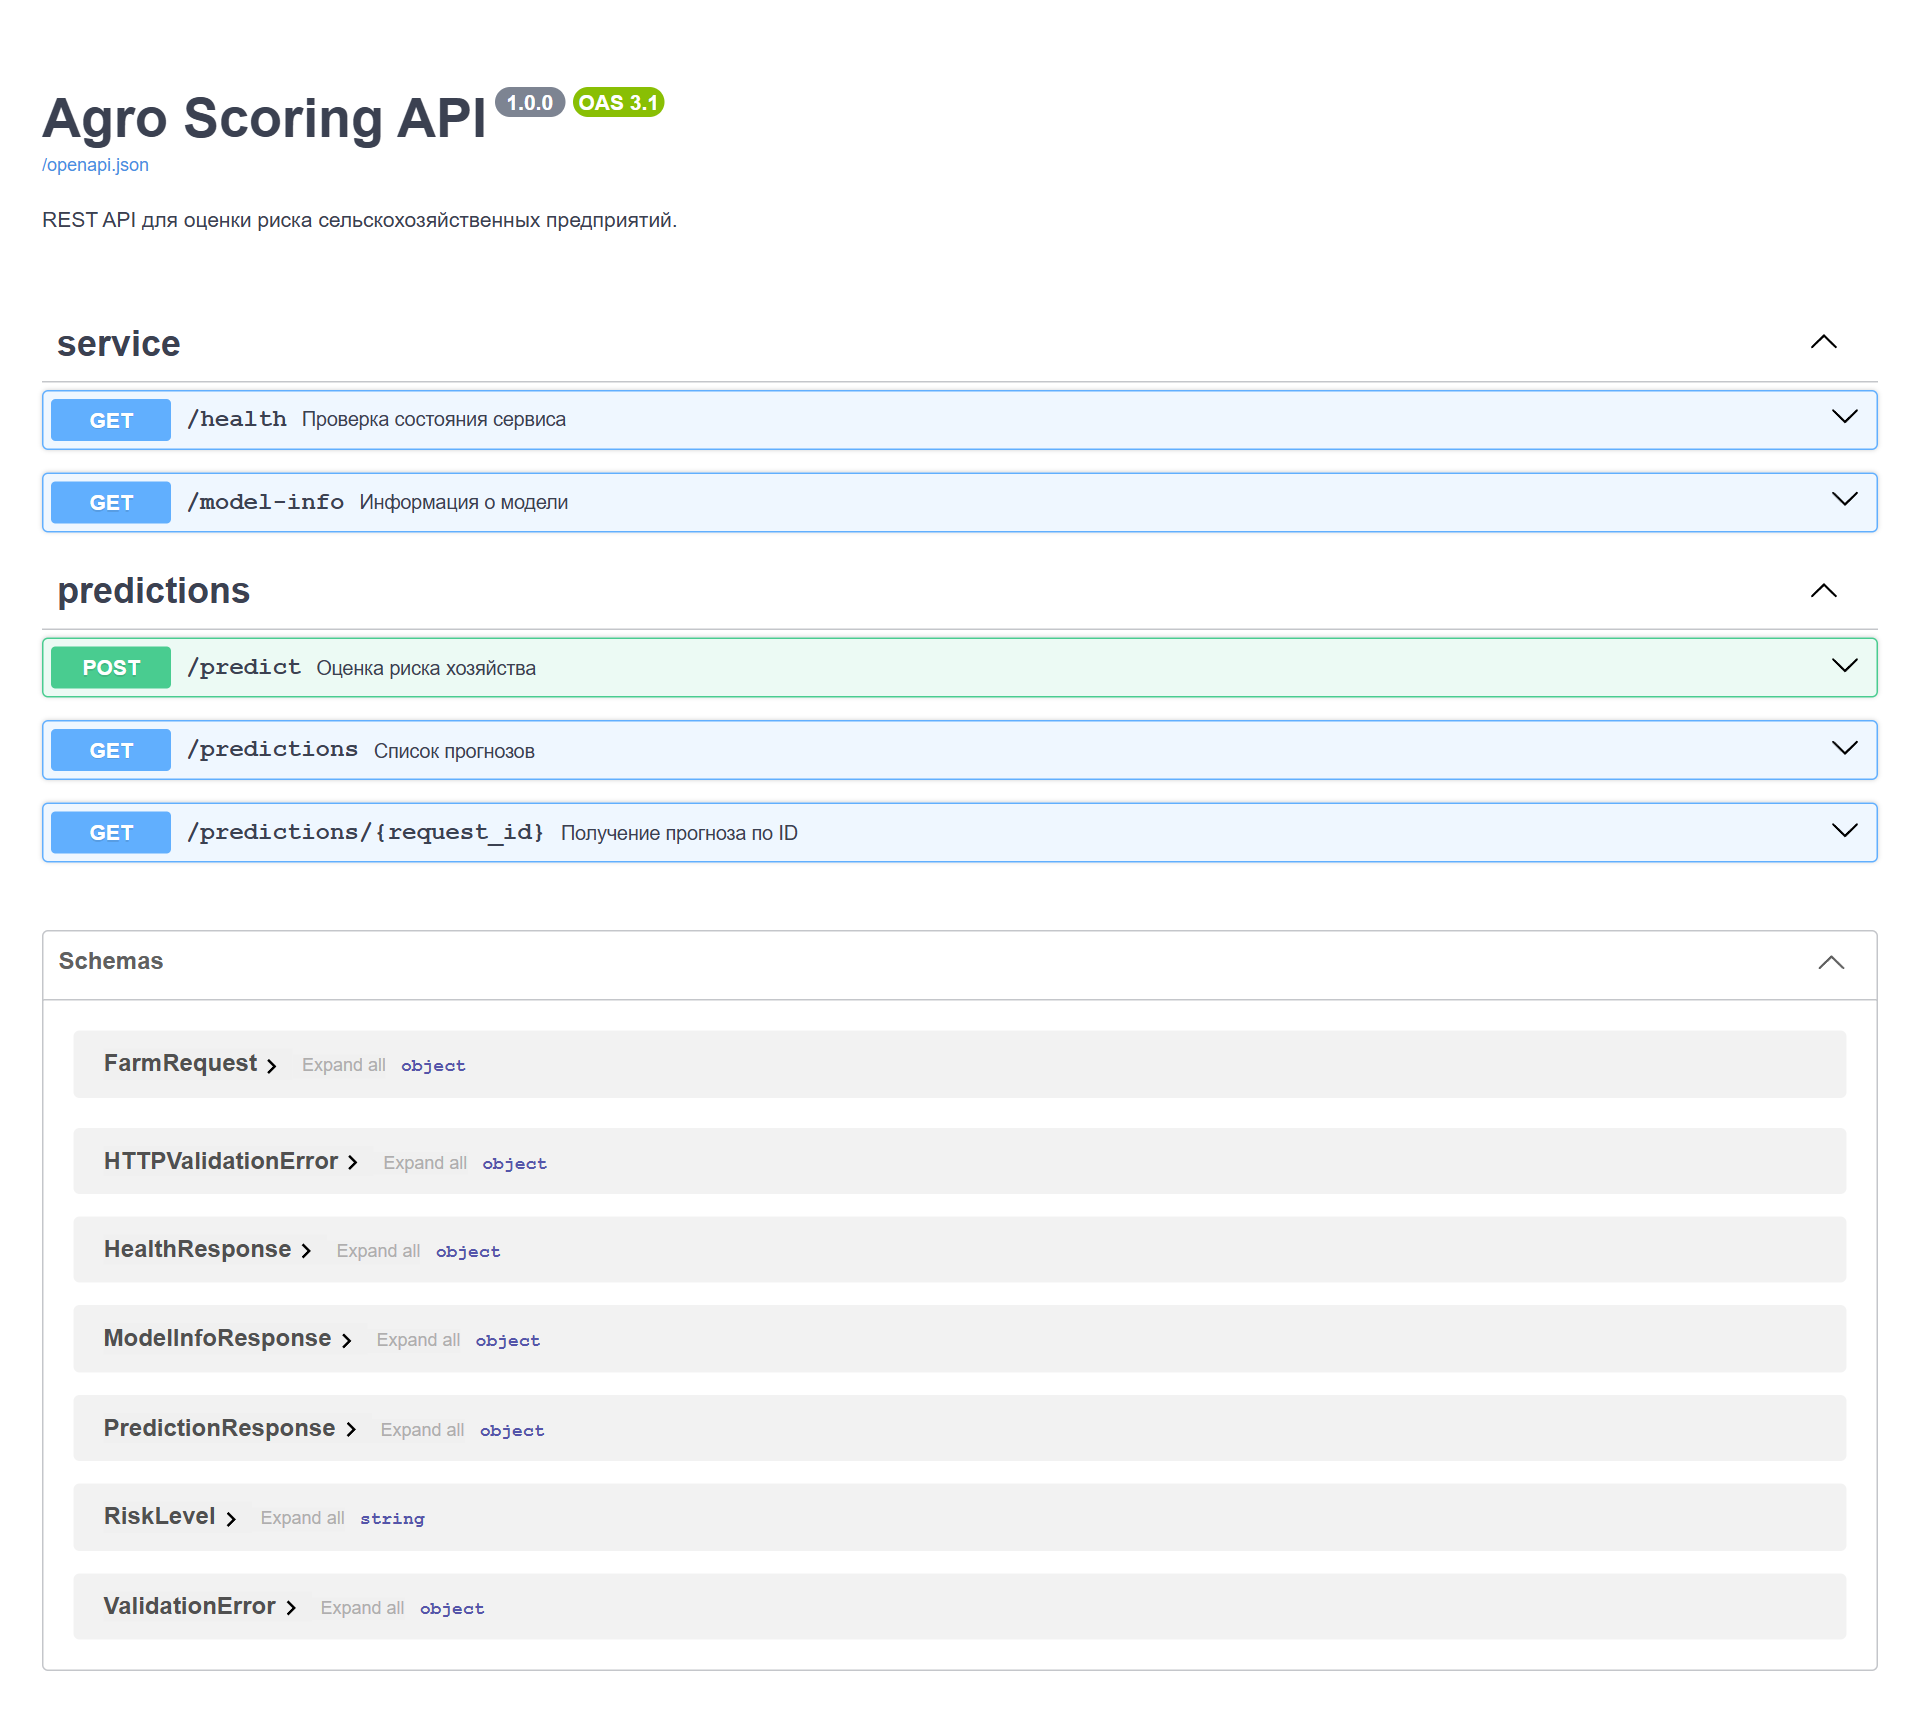
\includegraphics[width=0.85\textwidth]{img/swagger.png}
    \caption{Swagger UI: список endpoints и схем}
\end{figure}

\begin{figure}[H]
    \centering
    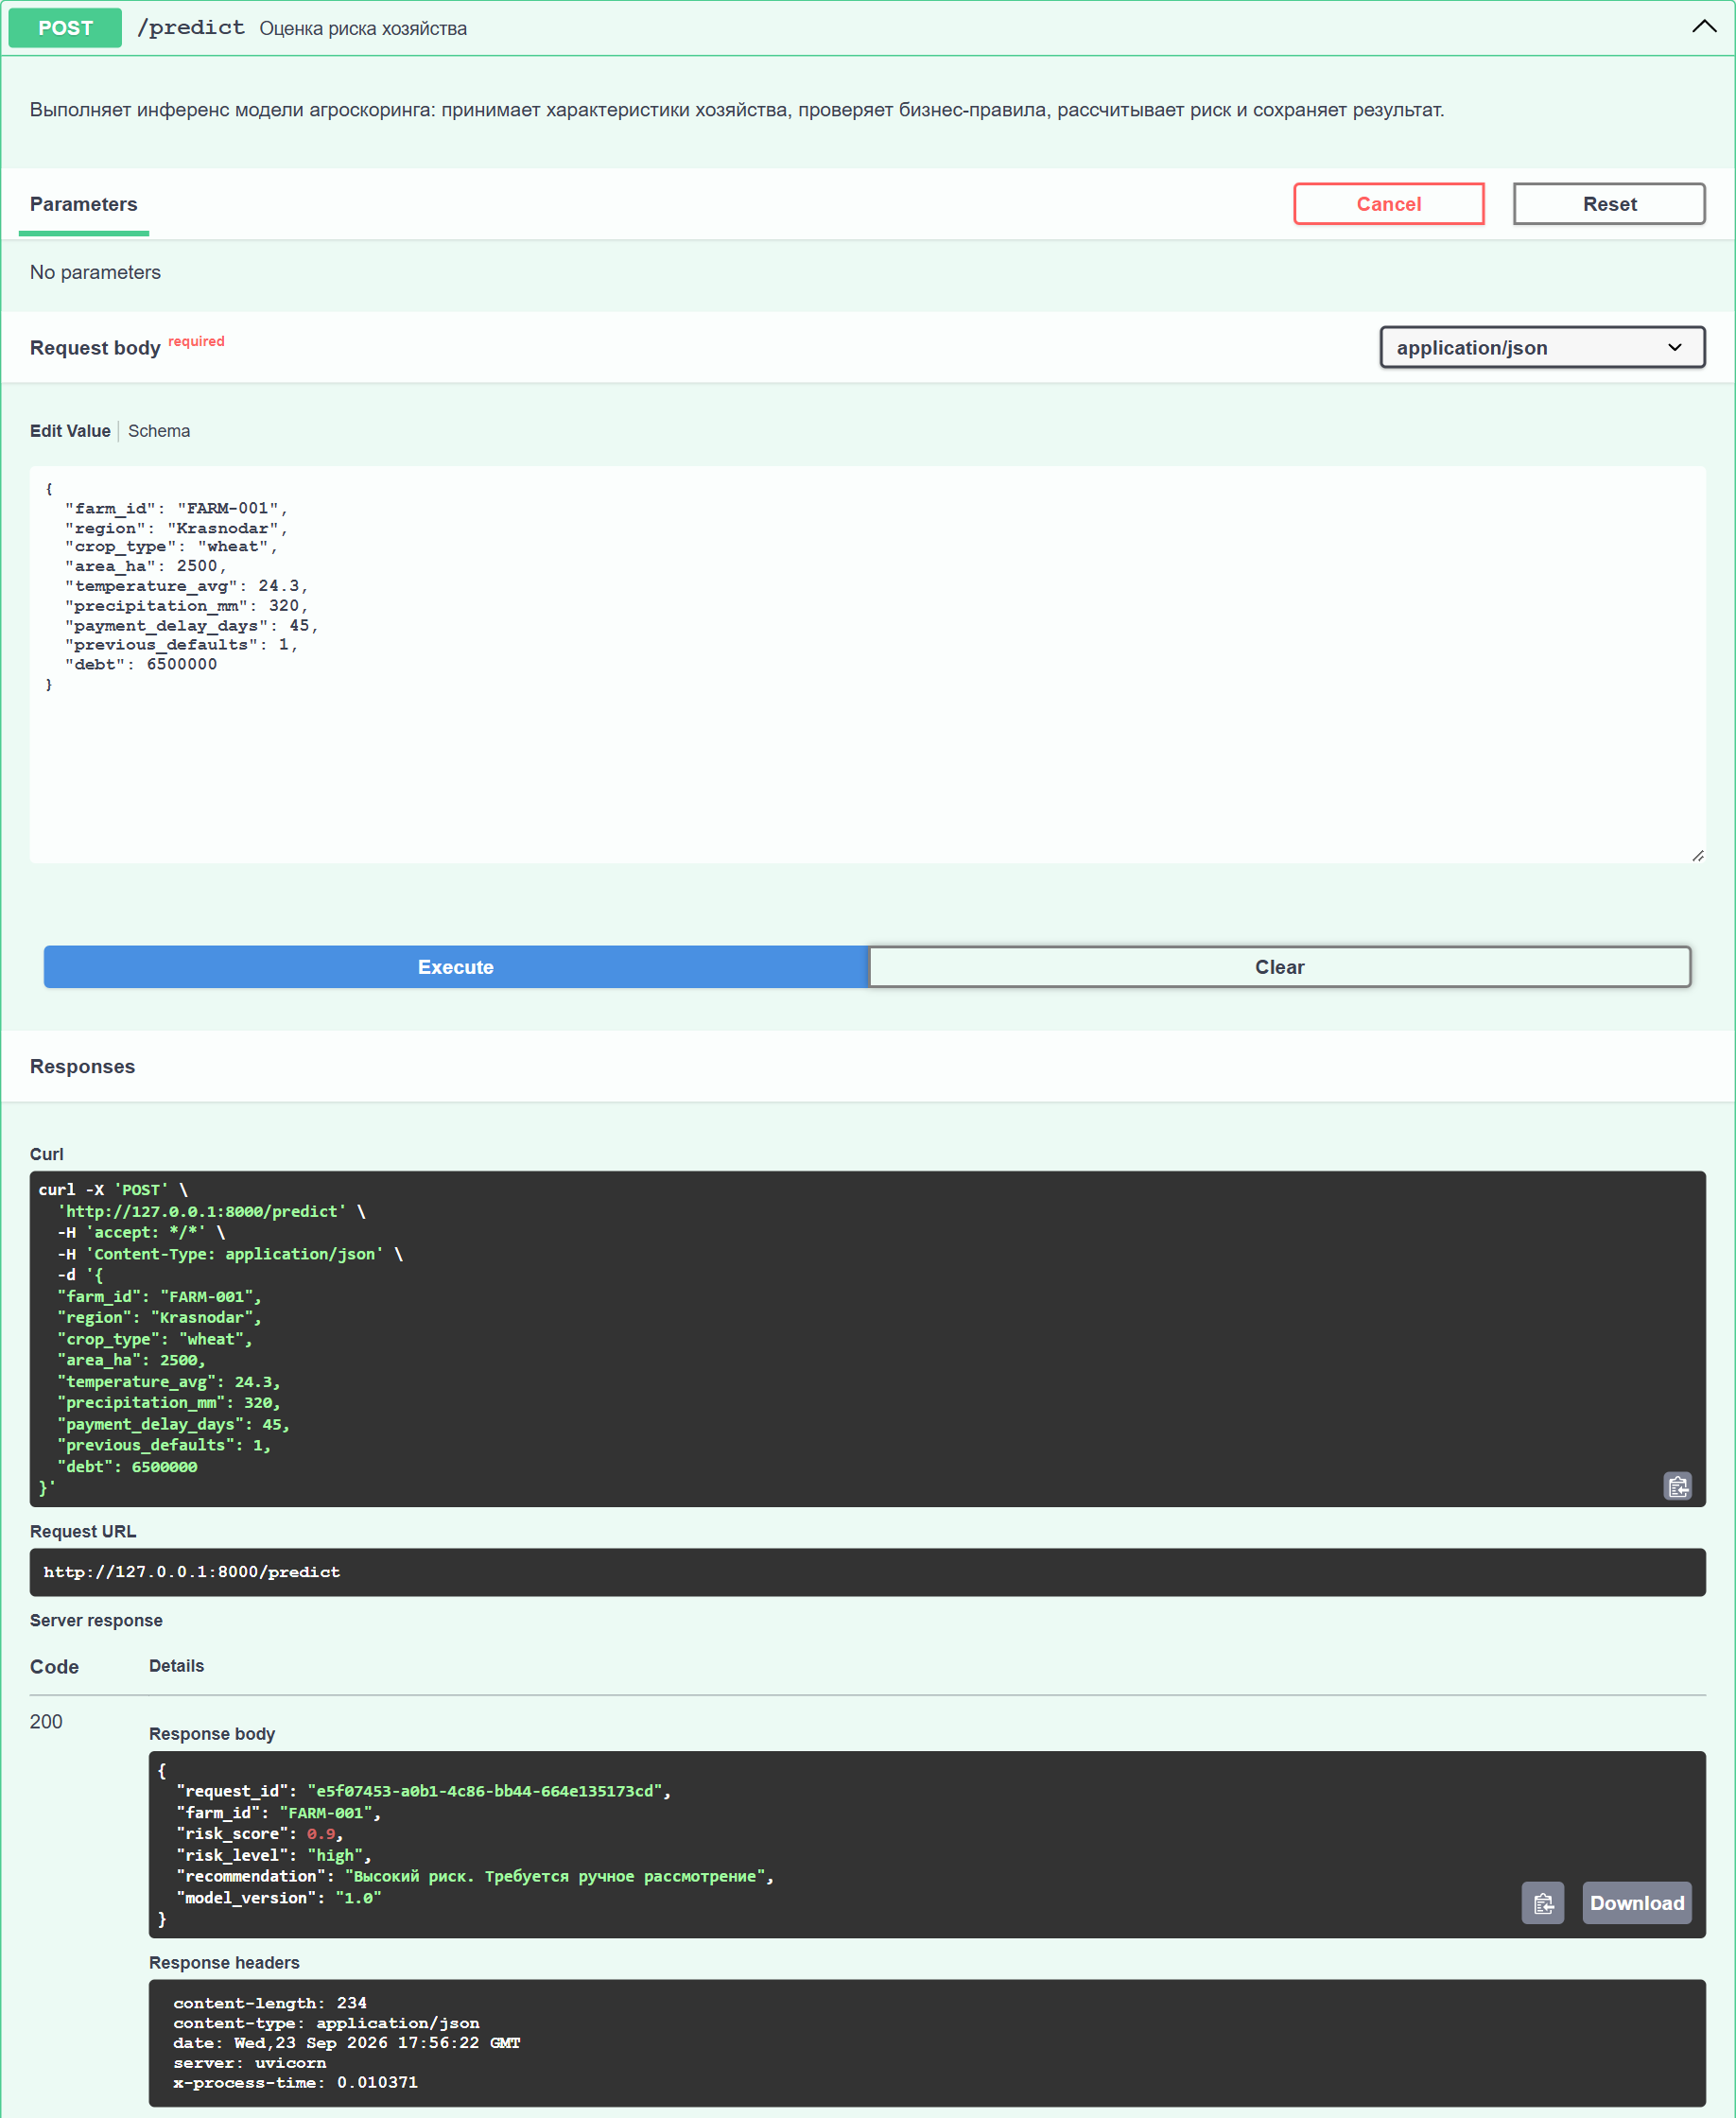
\includegraphics[width=0.8\textwidth]{img/predict_ok.png}
    \caption{Успешный запрос POST /predict (200 OK)}
\end{figure}

\begin{figure}[H]
    \centering
    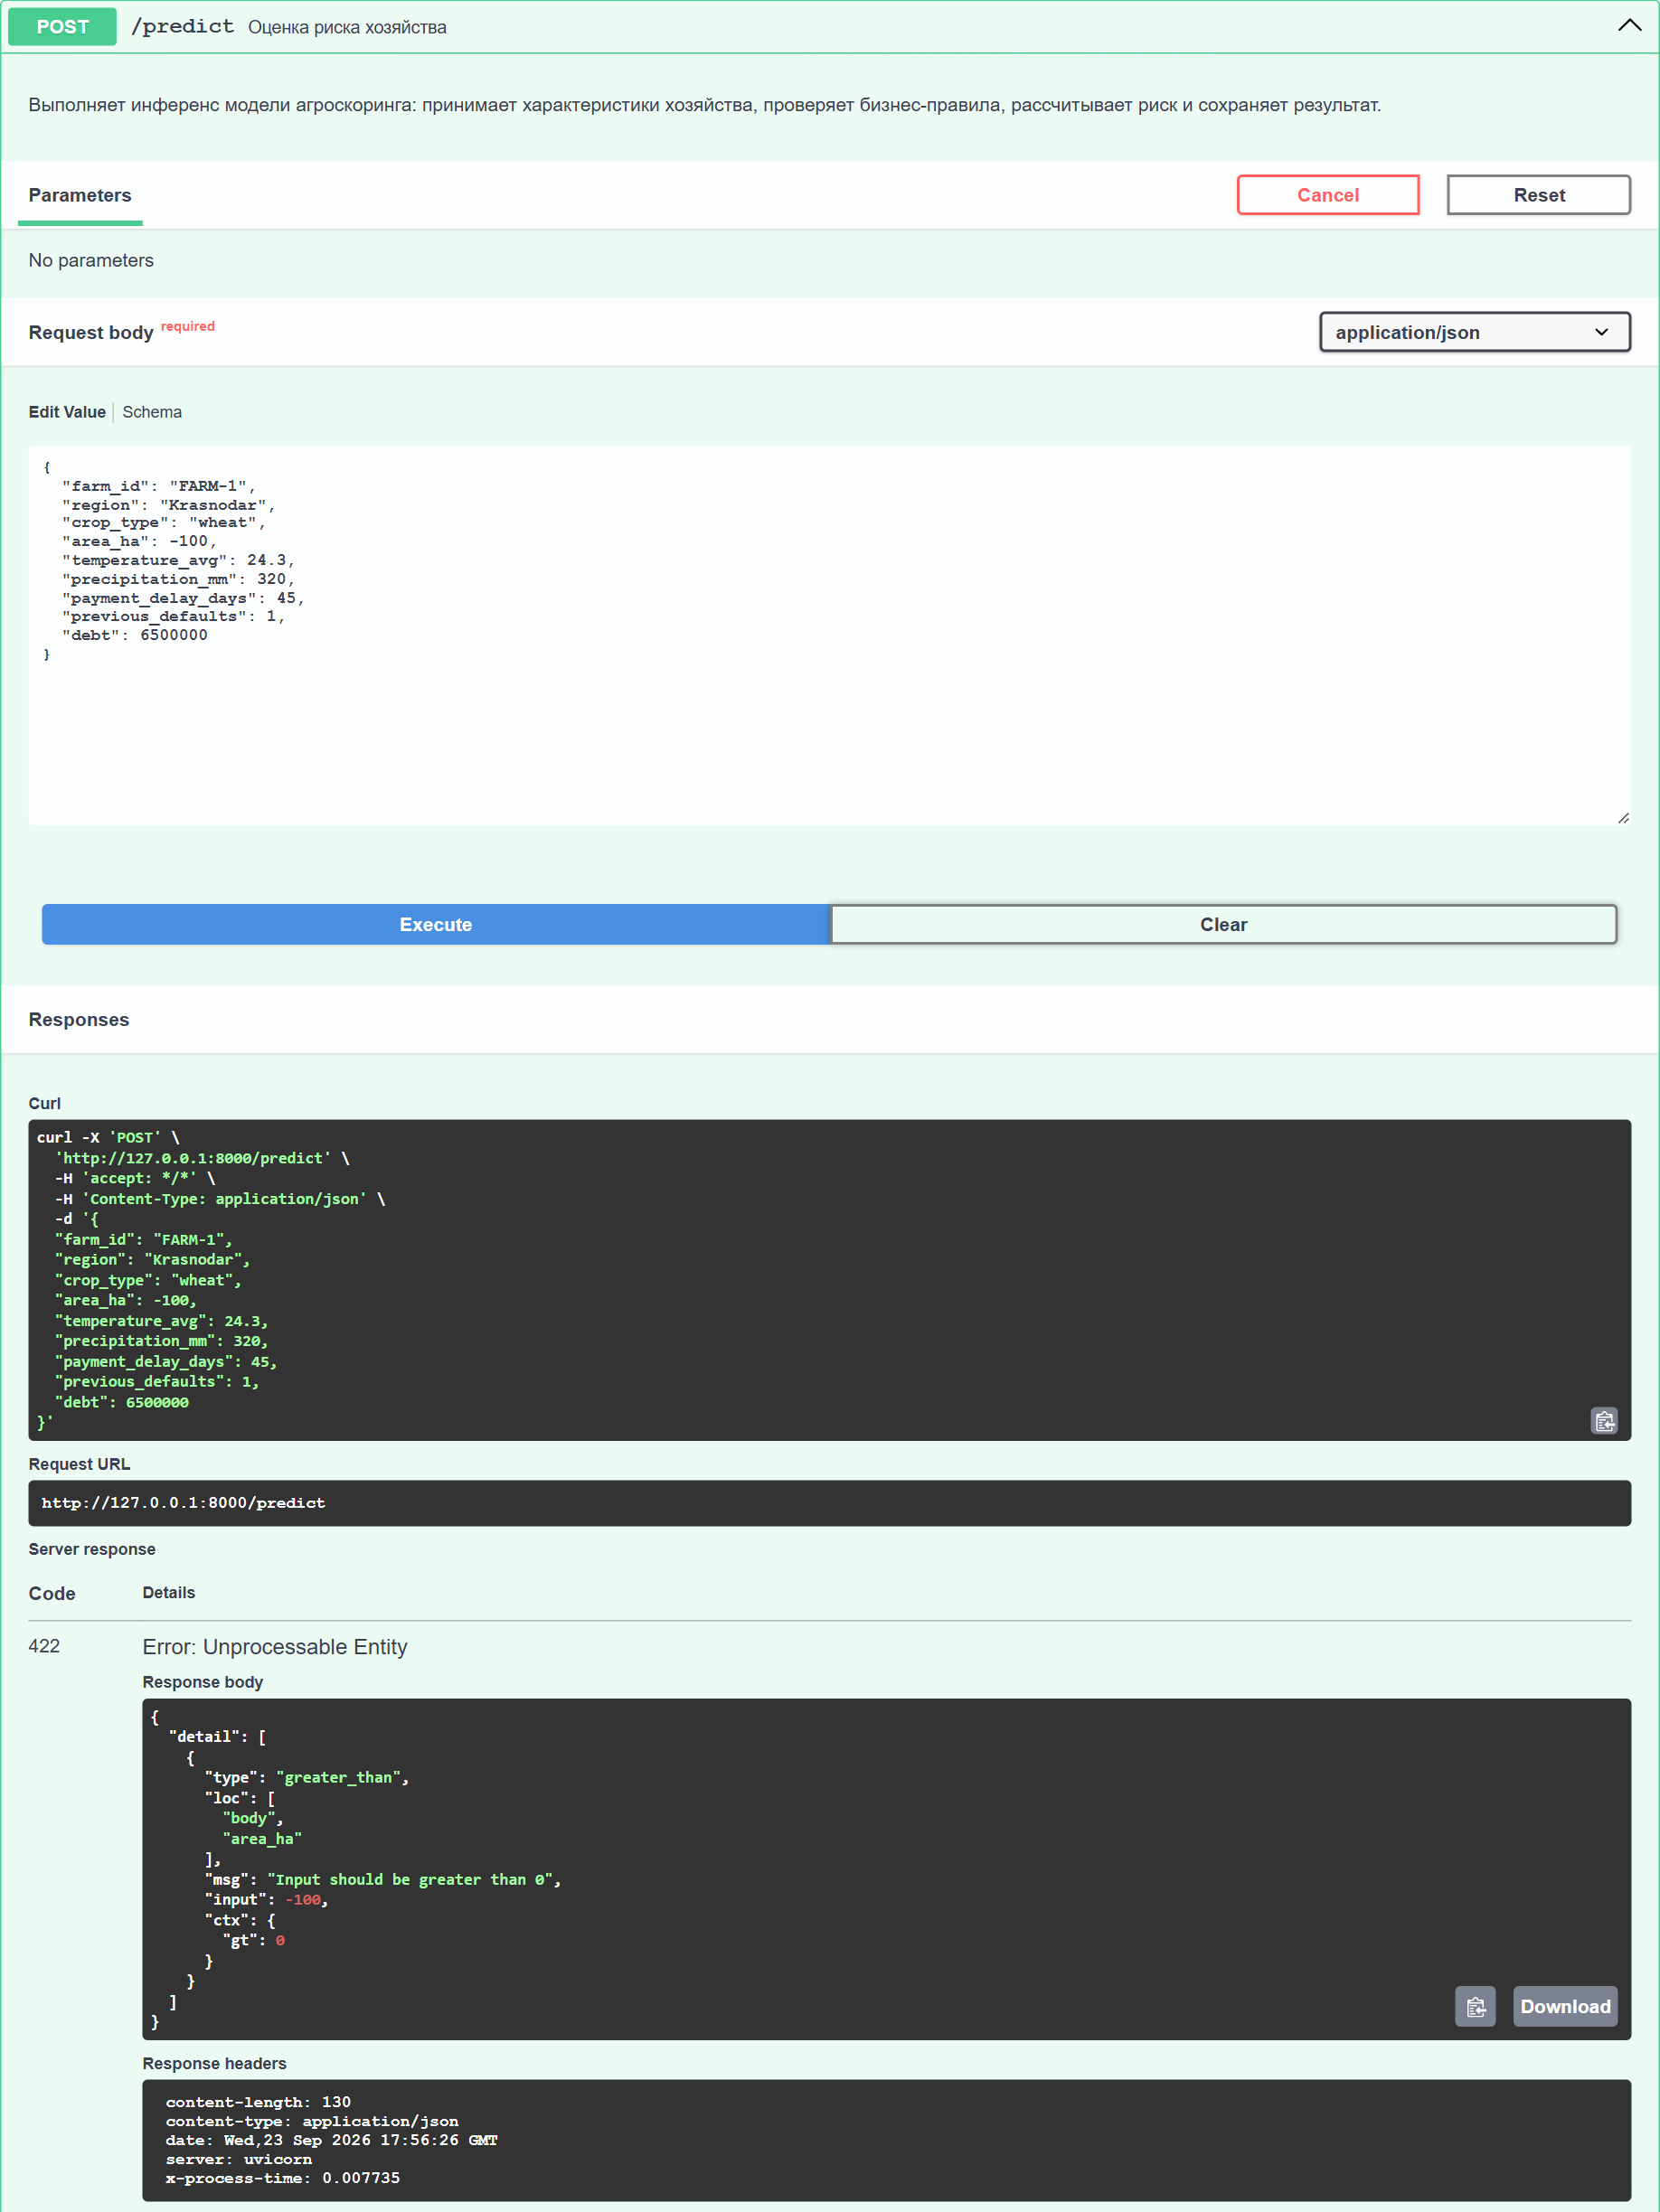
\includegraphics[width=0.8\textwidth]{img/predict_422.png}
    \caption{Ошибка валидации Pydantic: \texttt{area\_ha = -100} (422 Unprocessable Entity)}
\end{figure}

Ответ 422 содержит массив \texttt{detail}, в котором для каждой ошибки указаны: \texttt{type} (тип нарушения, здесь \texttt{greater\_than}), \texttt{loc} (где ошибка: \verb|["body", "area_ha"]|), \texttt{msg} (текстовое описание), \texttt{input} (переданное значение) и \texttt{ctx} (нарушенное ограничение, \texttt{gt: 0}). Клиент по этому ответу точно знает, какое поле исправить.

\begin{figure}[H]
    \centering
    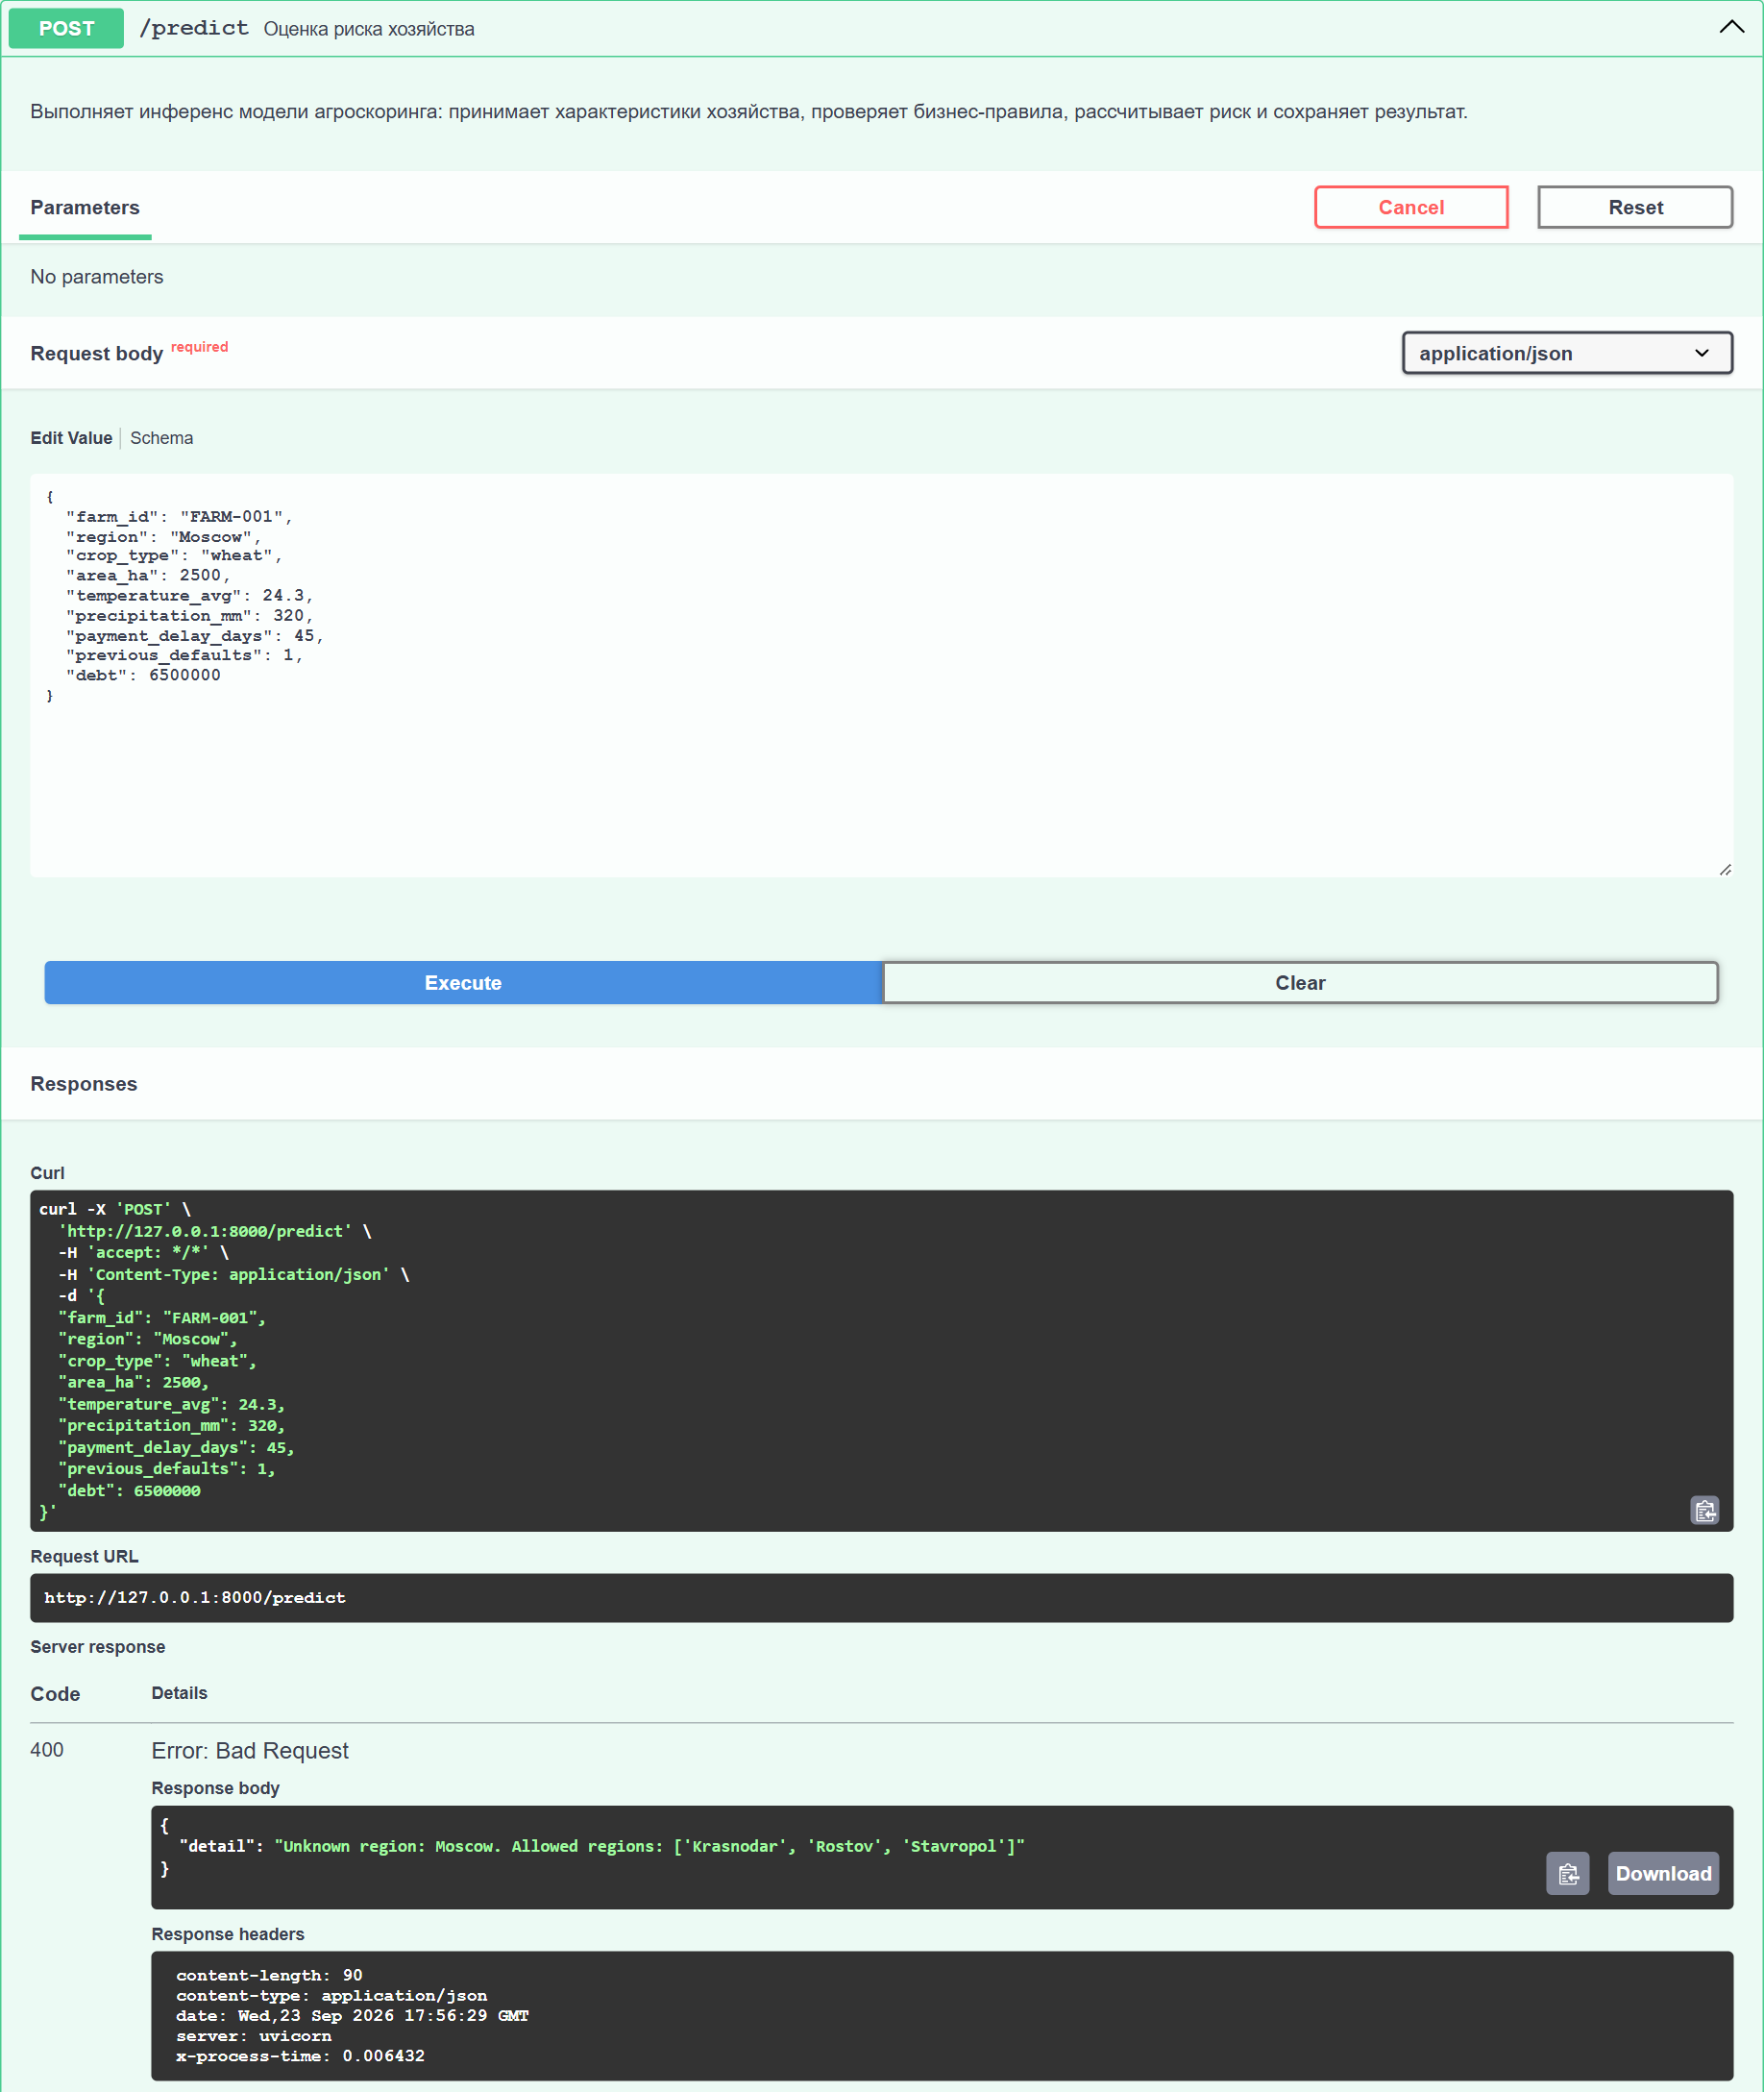
\includegraphics[width=0.8\textwidth]{img/predict_400.png}
    \caption{Бизнес-валидация: неизвестный регион (400 Bad Request)}
\end{figure}

\begin{figure}[H]
    \centering
    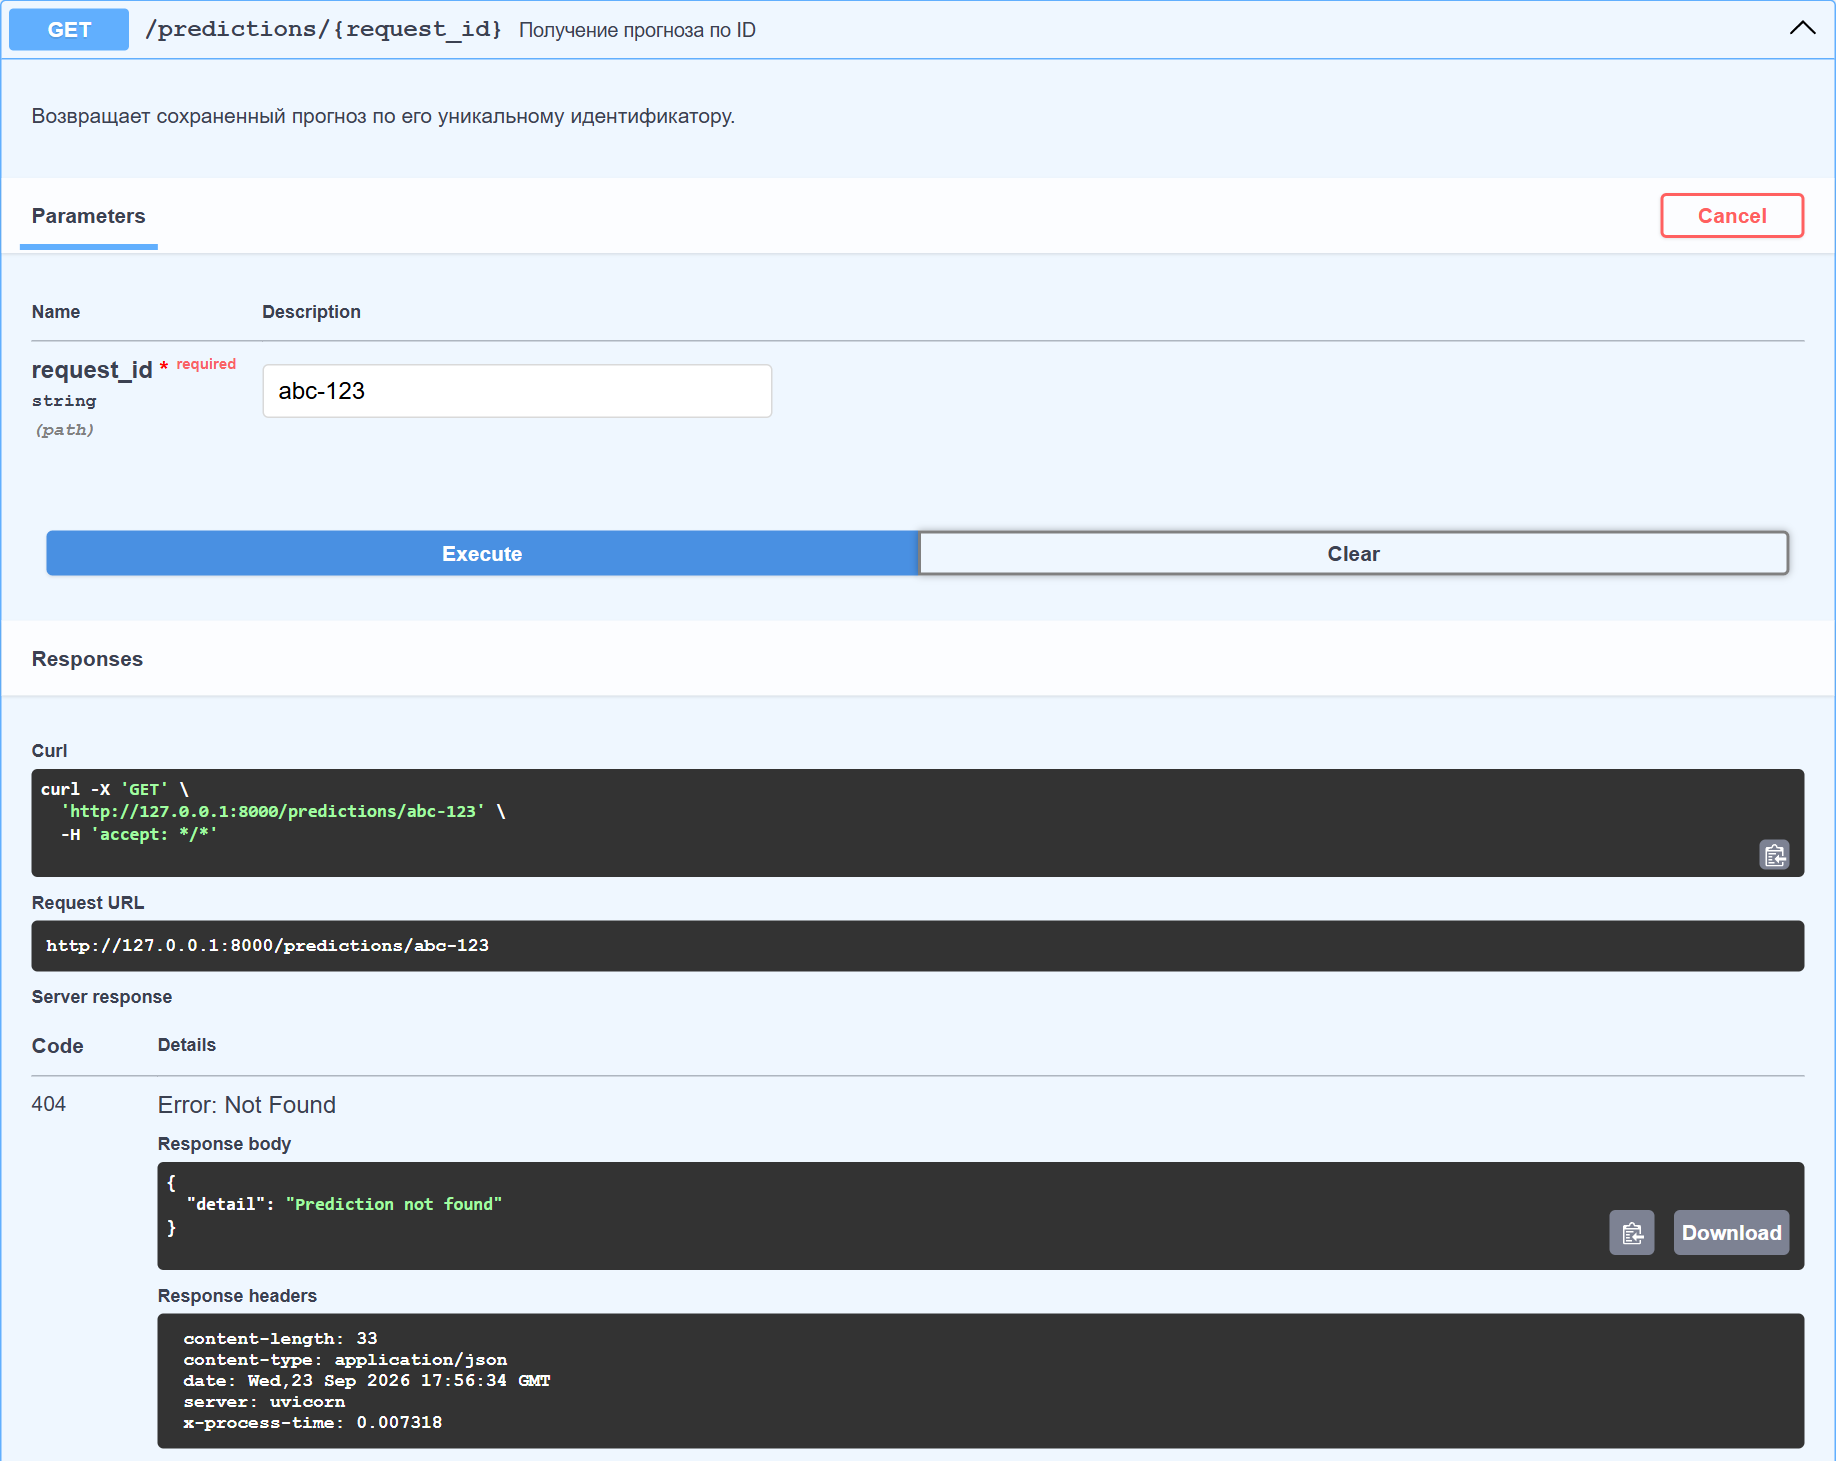
\includegraphics[width=0.8\textwidth]{img/get_404.png}
    \caption{Запрос несуществующего прогноза (404 Not Found)}
\end{figure}

\begin{figure}[H]
    \centering
    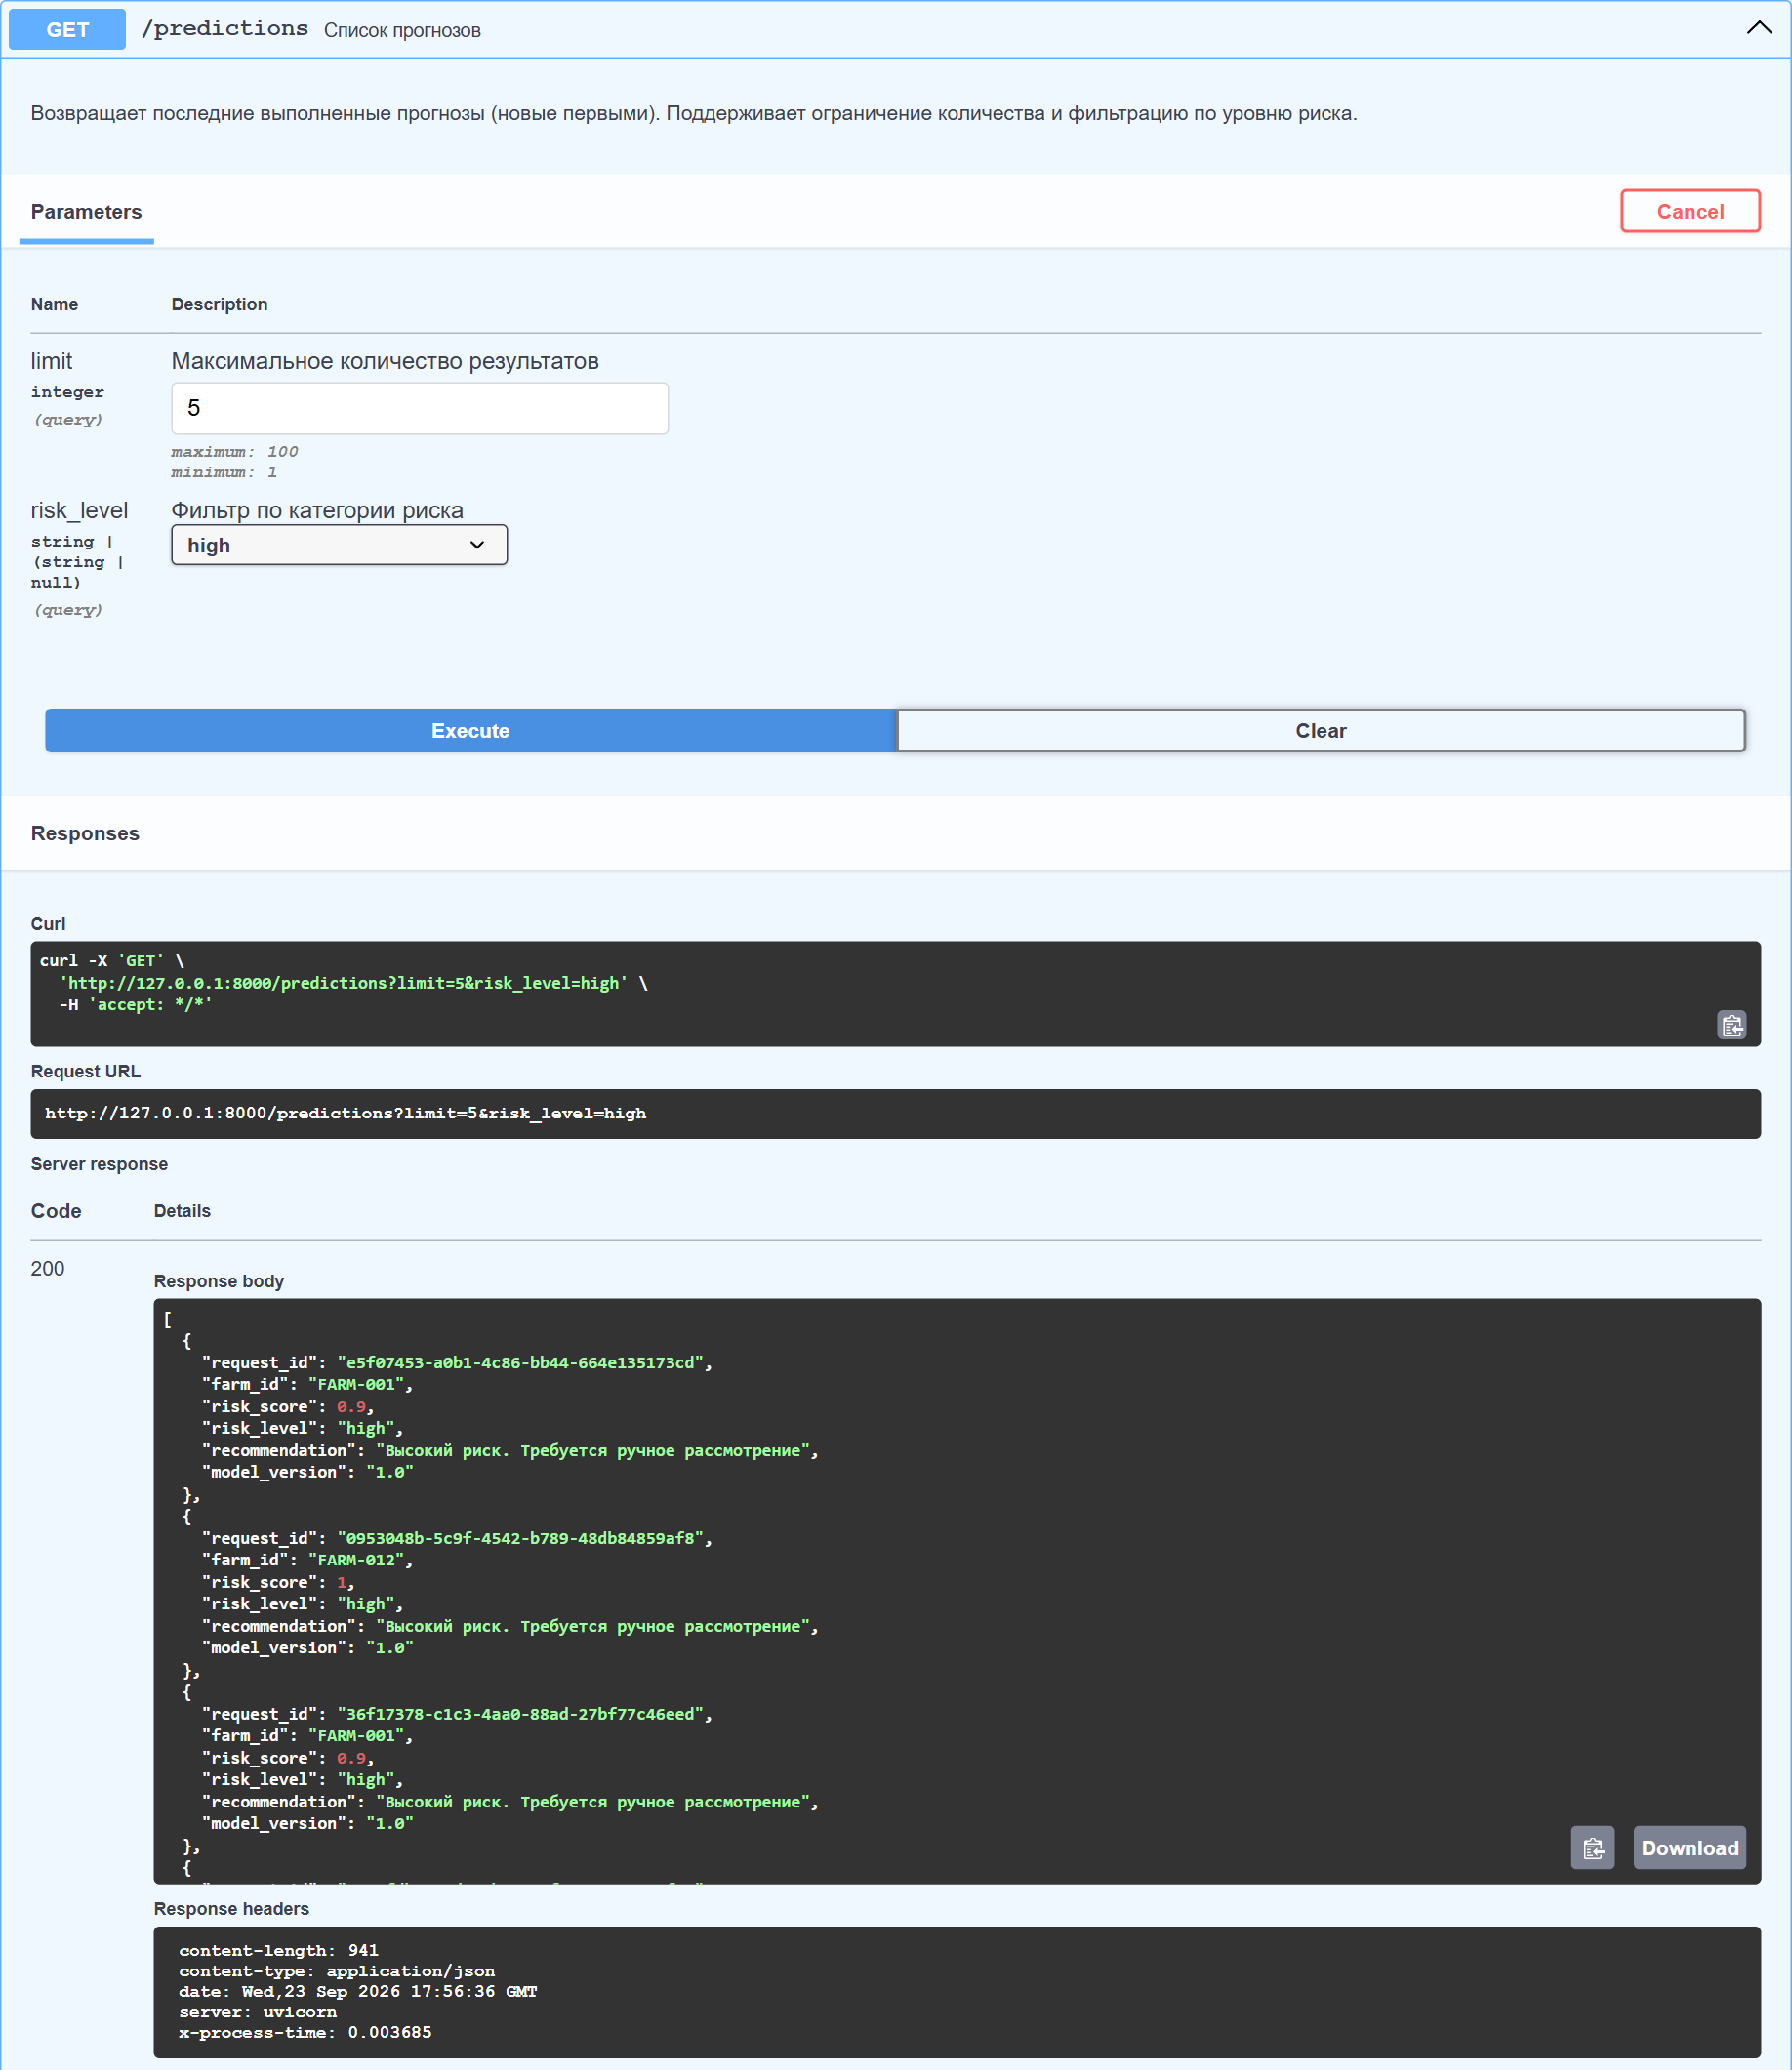
\includegraphics[width=0.8\textwidth]{img/list_high.png}
    \caption{Список прогнозов с фильтром \texttt{risk\_level=high} и \texttt{limit=5}}
\end{figure}

% ============================================================
\section{Таблица тест-кейсов}

Запросы выполнены к запущенному серверу (\texttt{uvicorn}); те же сценарии автоматизированы в \texttt{tests/test\_api.py} (15 HTTP-тестов). Логика модели, постпроцессинга, бизнес-правил и сервисов проверяется модульными тестами в \texttt{tests/test\_domain.py} (16 тестов). Все 31 тест пройдены.

\begin{table}[H]
\centering
\caption{Таблица тест-кейсов}
\begin{tabular}{|c|p{6.2cm}|c|c|c|}
\hline
\textbf{№} & \textbf{Запрос} & \textbf{Ожидаемый} & \textbf{Полученный} & \textbf{Результат} \\
\hline
1  & GET /health & 200 & 200 & пройден \\
2  & GET /model-info & 200 & 200 & пройден \\
3  & корректный POST /predict & 200 & 200 & пройден \\
4  & POST /predict, \texttt{area\_ha = -100} & 422 & 422 & пройден \\
5  & POST /predict, неизвестный регион & 400 & 400 & пройден \\
6  & GET /predictions/\{существующий id\} & 200 & 200 & пройден \\
7  & GET /predictions/\{неизвестный id\} & 404 & 404 & пройден \\
8  & GET /predictions?limit=2 & 200 & 200 & пройден \\
9  & GET /predictions?risk\_level=high & 200 & 200 & пройден \\
10 & GET /predictions?limit=-5 & 422 & 422 & пройден \\
\hline
\end{tabular}
\end{table}

% ============================================================
\section{Анализ API как контракта}

\begin{table}[H]
\centering
\caption{API-контракт}
\small
\begin{tabular}{|p{3.3cm}|p{1.2cm}|p{2.6cm}|p{3.3cm}|p{1.3cm}|p{2.3cm}|}
\hline
\textbf{Endpoint} & \textbf{Method} & \textbf{Input} & \textbf{Output} & \textbf{Success} & \textbf{Ошибки} \\
\hline
/health & GET & --- & HealthResponse & 200 & 500 \\
/model-info & GET & --- & ModelInfoResponse & 200 & 500 \\
/predict & POST & body: FarmRequest & PredictionResponse & 200 & 400, 422, 503, 500 \\
/predictions/\{request\_id\} & GET & path: request\_id & PredictionResponse & 200 & 404, 500 \\
/predictions & GET & query: limit, risk\_level & list[PredictionResponse] & 200 & 422, 500 \\
\hline
\end{tabular}
\end{table}

Каждый endpoint имеет явную схему ответа (\texttt{response\_model}), поэтому клиент получает предсказуемую структуру независимо от внутреннего устройства модели, а лишние внутренние поля не попадают в ответ. Возможные коды ошибок (400, 404, 503) дополнительно описаны в параметре \texttt{responses} и отображаются в Swagger UI.

% ============================================================
\section{Ответы на вопросы}

\subsection{Чем /health отличается от /model-info?}

\texttt{/health} отвечает на вопрос «жив ли процесс API и принимает ли он HTTP-запросы». Это лёгкая проверка без обращения к модели и хранилищу; её используют балансировщик нагрузки, системы мониторинга и оркестратор (liveness probe), вызывая часто и автоматически.

\texttt{/model-info} отвечает на вопрос «какая модель обслуживает запросы и готова ли она». Он возвращает метаданные: имя, версию, тип и статус модели. Это нужно клиентам и аналитикам (какая версия дала прогноз), для аудита и для проверки готовности (readiness): API может быть жив (\texttt{/health} = ok), а модель --- ещё не загружена (\texttt{status = unavailable}).

\subsection{Почему некорректный запрос не должен доходить до ML-модели?}

\begin{itemize}
    \item Модель не понимает физического смысла признаков: на отрицательной площади или отрицательном долге она не упадёт, а выдаст правдоподобное, но бессмысленное число (garbage in --- garbage out), и банк примет решение на основе мусора.
    \item Некорректные типы или пропущенные поля могут вызвать исключение внутри модели и ответ 500, который не объясняет клиенту, что исправить.
    \item Ошибочный результат попадёт в хранилище и логи, искажая статистику и мониторинг качества модели.
    \item Расчёт прогноза --- самая дорогая операция; отсекать ошибки нужно как можно раньше (принцип fail fast).
    \item Ответ 422 с указанием поля и нарушенного ограничения --- часть контракта: клиент понимает, что проблема в его данных и повтор без исправления бесполезен.
\end{itemize}

\subsection{Какой статус корректнее для запроса на прогноз: 200 OK или 201 Created?}

Выбран \textbf{200 OK}, и он используется последовательно. \texttt{POST /predict} семантически является вычислением: клиент передаёт данные и сразу получает результат в теле ответа. Код 201 Created означает создание нового ресурса и по стандарту HTTP должен сопровождаться заголовком \texttt{Location} с адресом ресурса.

Аргумент в пользу 201 тоже существует: результат сохраняется и становится доступен по \texttt{/predictions/\{request\_id\}}. Если бы API проектировался как ресурсный (\texttt{POST /predictions}), 201 с \texttt{Location} был бы уместен. При переходе к асинхронной обработке корректным стал бы код 202 Accepted.

% ============================================================
\section{Вывод}

\begin{figure}[H]
    \centering
    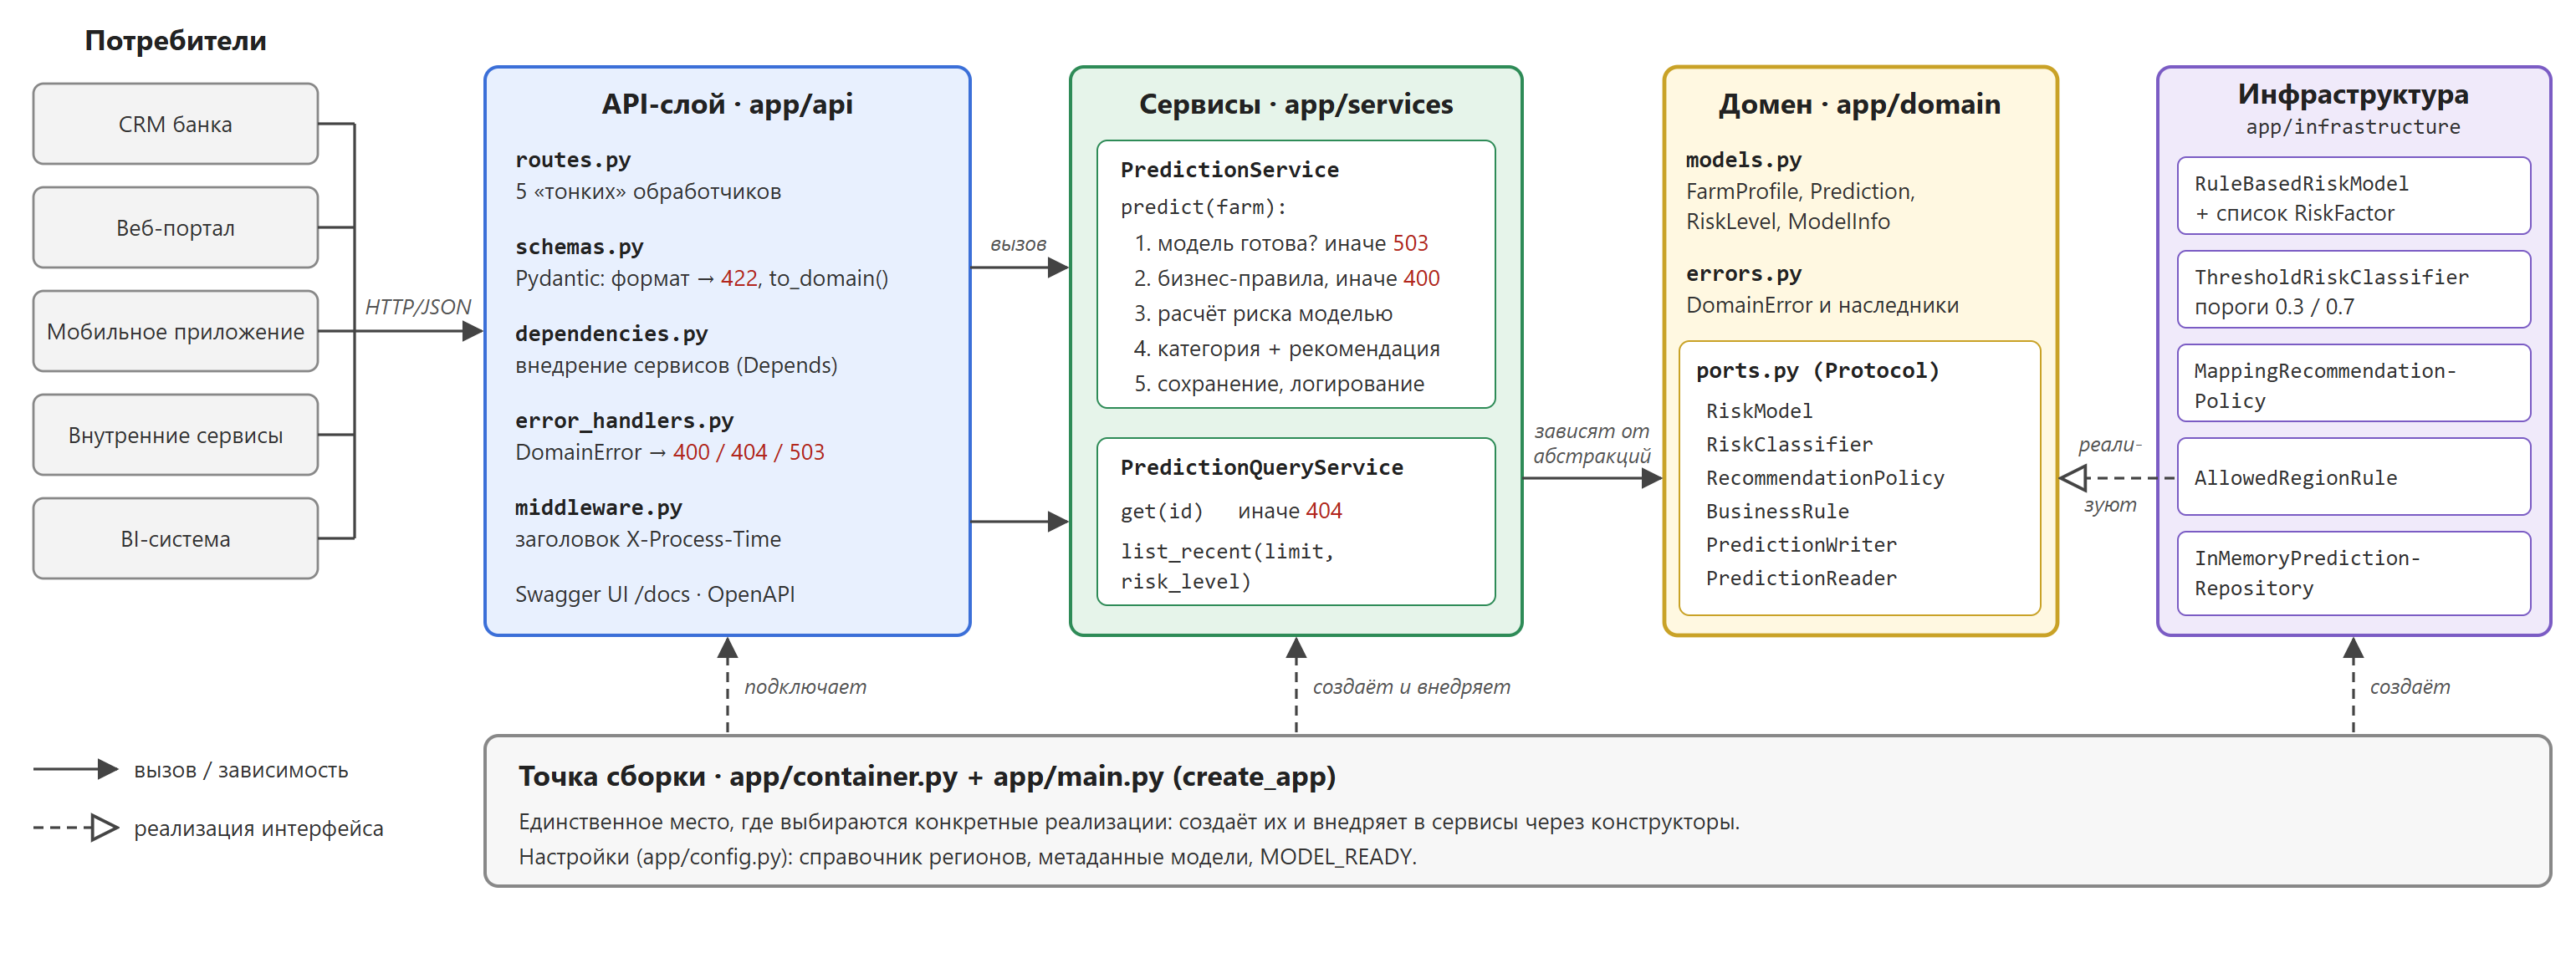
\includegraphics[width=\textwidth]{img/architecture_components.png}
    \caption{Компонентная схема архитектуры AI-сервиса агроскоринга}
    \label{fig:arch}
\end{figure}

В ходе работы разработан прототип REST API сервиса агроскоринга на FastAPI. Архитектура построена по слоям в соответствии с принципами SOLID. API-слой принимает HTTP-запросы, выполняет структурную валидацию Pydantic и переводит доменные ошибки в HTTP-коды. Сервисный слой реализует сценарии расчёта и чтения прогнозов и зависит только от абстракций предметной области. Инфраструктура содержит конкретные реализации: модель на правилах, постпроцессинг, бизнес-правила и хранилище. Все реализации подключаются в одной точке сборки, поэтому любую из них можно заменить без изменения остального кода.

Реализованы все пять требуемых endpoints, структурная (Pydantic, 422) и бизнес-валидация (400), обработка 404 и 503, path- и query-параметры, описания для OpenAPI. Все тест-кейсы пройдены. Бизнес-логика дополнительно покрыта модульными тестами, которые выполняются без HTTP: вместо модели и хранилища в сервис подставляются тестовые реализации.

REST API в AI-системе выполняет роль единой точки входа, изолятора и контракта. Он скрывает от потребителей (CRM, портал, мобильное приложение, BI) детали реализации модели --- фреймворк, версию, способ загрузки --- и предоставляет стабильный, документированный (OpenAPI) интерфейс с явными схемами данных и кодами ошибок. Благодаря этому модель можно переобучить, заменить на настоящую ML-модель или перенести на другой сервер, не меняя код клиентов, а валидация на уровне API защищает модель от некорректных данных.

\end{document}
